%-----------------------------------------------------------------------------%
\chapter{\babDua}
%-----------------------------------------------------------------------------%

%-----------------------------------------------------------------------------%
\section{Profil dan Sejarah Perusahaan}
%-----------------------------------------------------------------------------%

\subsection{Profil Perusahaan}
\namaUniv, yang umum dikenal juga sebagai Taiwan Tech, adalah salah satu institusi pendidikan di Taiwan yang berfokus pada riset dan perkembangan di bidang sains dan teknologi. Sejak didirikan pada tahun 1974, NTUST telah menjadi salah satu pusat pendidikan teknik dan teknologi utama di Taiwan.

NTUST berkolaborasi aktif dengan berbagai universitas lain dan industri dari seluruh dunia. Selain itu, NTUST juga berperan aktif dalam program-program pertukaran pendidikan internasional, seperti Taiwan Experience Education Program (TEEP), yang memberikan kesempatan kepada mahasiswa internasional untuk berpartisipasi dalam pendidikan dan penelitian yang komprehensif di Taiwan.

\subsection{Sejarah Perusahaan}
NTUST didirikan pada tahun 1974 sebagai lembaga pendidikan tinggi pertama di Taiwan yang khusus didedikasikan untuk pendidikan teknologi dan teknik. Awalnya didirikan sebagai ``National Taiwan Institute of Technology'' (NTIT), universitas ini bertujuan untuk memenuhi kebutuhan Taiwan akan tenaga kerja yang terampil di bidang teknologi, seiring dengan pesatnya pertumbuhan industri di negara tersebut.

Sejak pendiriannya, NTUST telah mengalami berbagai transformasi signifikan. Pada tahun 1981, universitas ini dinaikkan statusnya menjadi universitas teknologi pertama di Taiwan dan kemudian berganti nama menjadi \namaUniv. Sejak itu, NTUST telah berkembang pesat, memperluas program akademiknya untuk mencakup berbagai bidang.

%-----------------------------------------------------------------------------%
\section{Kegiatan/Bidang Usaha Perusahaan}
%-----------------------------------------------------------------------------%

Kegiatan utama NTUST meliputi penyelenggaraan program-program akademik yang mencakup berbagai bidang seperti Teknik Elektro, Ilmu Komputer, Teknik Industri, dan Teknologi Informasi. Universitas ini menyediakan pendidikan berkualitas tinggi melalui program sarjana, magister, dan doktoral yang dirancang untuk memenuhi tuntutan industri dan perkembangan teknologi terkini.

Dalam hal penelitian, NTUST berkomitmen untuk melakukan penelitian terdepan dalam berbagai bidang teknologi yang terus berkembang, termasuk teknik elektro, ilmu komputer, teknik industri, dan manajemen teknologi. Penelitian di NTUST dilakukan di berbagai laboratorium dan pusat riset yang dilengkapi dengan fasilitas modern, mendukung kegiatan riset dasar maupun terapan yang dapat memberikan kontribusi langsung bagi kemajuan teknologi.

NTUST juga aktif dalam menjalin kerja sama dengan industri dan institusi penelitian lainnya, baik di tingkat nasional maupun internasional. Melalui kolaborasi ini, NTUST mengaplikasikan hasil penelitian dalam konteks praktis dan memberikan solusi inovatif untuk tantangan teknologi. Kegiatan ini mencakup pengembangan teknologi baru, evaluasi yang sudah ada, dan pemecahan masalah yang relevan dengan kebutuhan industri modern.

%-----------------------------------------------------------------------------%
\section{Lokasi Perusahaan}
%-----------------------------------------------------------------------------%

Program TEEP diadakan di \namaUniv \ , dilaksanakan di gedung CEECS (College of Electrical Engineering and Computer Science) yang berlokasi di No. 43, Section 4, Keelung Road, Da'an District, Taipei City, Taiwan 106. Lokasi ini ada di pusat kota Taipei dengan akses transportasi yang dekat dengan berbagai fasilitas pendukung.

% \begin{figure}[H]
%     \centering
%     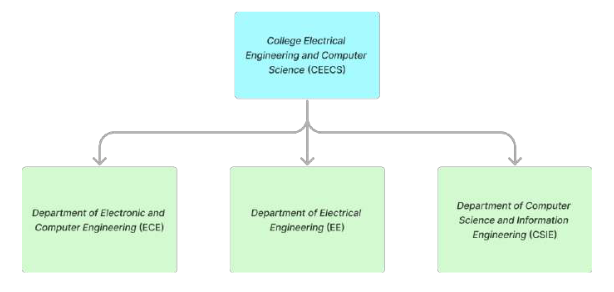
\includegraphics[width=0.6\textwidth]{assets/pics/ceecs.png}
%     \caption{Peta Lokasi NTUST}
%     \label{fig:lokasi_ntust}
% \end{figure}

\begin{figure}[H]
    \centering
    
\includegraphics[width=0.8\textwidth]{assets/pics/bmw.jpg}
    \caption{Logo \namaLab}
    \label{fig:logo_bmw}
\end{figure}

%-----------------------------------------------------------------------------%
\section{Struktur Organisasi Perusahaan}
%-----------------------------------------------------------------------------%

\textit{College of Electrical Engineering and Computer Science} (CEECS) di NTUST didirikan pada Agustus 1998 untuk mendidik mahasiswa dalam profesi di bidang teknik listrik, teknik elektronik, dan ilmu komputer. Berkomitmen untuk menjadi lembaga penelitian yang diakui secara internasional, CEECS telah mengejar pendidikan dengan kurikulum yang ketat dan penelitian tentang teknologi inovatif.

CEECS terdiri dari tiga departemen utama yaitu Departemen Teknik Elektronik dan Komputer, Departemen Teknik Elektro, dan Departemen Ilmu Komputer dan Teknik Informasi, serta satu lembaga pascasarjana yaitu Program Pascasarjana Teknik Elektro-Optik. Semua departemen ini menyediakan program doktoral dan magister dengan fokus penelitian yang berbeda-beda.

\begin{figure}[H]
    \centering
    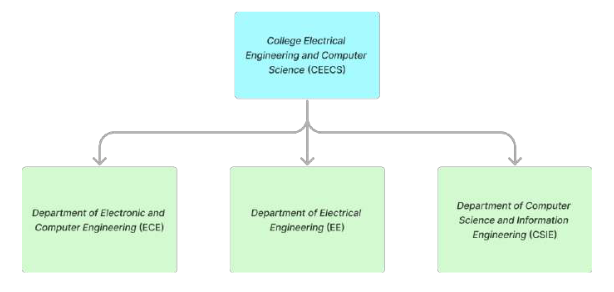
\includegraphics[width=0.8\textwidth]{assets/pics/ceecs.png}
    \caption{Struktur Organisasi CEECS}
    \label{fig:struktur_ceecs}
\end{figure}

Departemen Teknik Elektronik dan Komputer di CEECS didirikan bersamaan dengan NTUST yaitu pada tahun 1974. Pendirian departemen ini bertujuan untuk mendidik para insinyur dan peneliti yang berkualifikasi tinggi untuk industri elektronik dan optoelektronik yang berkembang pesat. Dalam beberapa tahun terakhir, departemen ini telah mencapai keunggulan di bidang \textit{embedded system}, desain \textit{chip} IC, jaringan nirkabel dan \textit{broadband}, komunikasi optik, serta bidang-bidang \textit{emerging technology} lainnya.

%-----------------------------------------------------------------------------%
\section{Profil \namaLab}
%-----------------------------------------------------------------------------%

Laboratorium BMW adalah pusat riset yang berfokus pada inovasi dalam teknologi komunikasi dan informasi. Laboratorium ini berfokus dalam bidang teknologi \textit{broadband}, \textit{multimedia}, dan \textit{wireless communication} dengan mendalami topik-topik penelitian yang mencakup optimisasi WiFi, \textit{5G Energy Saving}, dan \textit{Open Radio Access Network} (O-RAN).

\namaLab \ di NTUST ini menyediakan akses langsung ke sumber daya penelitian dan dukungan infrastruktur untuk penelitian dan pengembangan berkelanjutan. Laboratorium ini dilengkapi dengan fasilitas seperti \textit{server}, \textit{Radio Unit} (RU), dan \textit{computing infrastructure}, peralatan \textit{testing} dan \textit{measurement} untuk \textit{wireless communication}, \textit{software development tools} dan \textit{simulation environment}, serta \textit{testbed} untuk eksperimen jaringan yang memungkinkan validasi hasil penelitian secara \textit{real-time}.
